\documentclass{beamer}
\usepackage{color}
\usepackage{bm}
\usepackage{graphicx}
\usepackage{hyperref}
\usepackage{listings}
\beamertemplatenavigationsymbolsempty
\definecolor{mygreen}{rgb}{0,0.6,0}
\definecolor{mymauve}{rgb}{0.58,0,0.82}
\lstset{ %
  backgroundcolor=\color{white},   % choose the background color; you must add \usepackage{color} or \usepackage{xcolor}
  basicstyle=\footnotesize,        % the size of the fonts that are used for the code
  commentstyle=\color{mygreen},    % comment style
  deletekeywords={...},            % if you want to delete keywords from the given language
  extendedchars=true,              % lets you use non-ASCII characters; for 8-bits encodings only, does not work with UTF-8
  frame=single,                    % adds a frame around the code
  keywordstyle=\color{blue},       % keyword style
  language=Python,                 % the language of the code
  rulecolor=\color{black},         % if not set, the frame-color may be changed on line-breaks within not-black text (e.g. comments (green here))
  showspaces=false,                % show spaces everywhere adding particular underscores; it overrides 'showstringspaces'
  stringstyle=\color{mymauve},     % string literal style
  title=\lstname                   % show the filename of files included with \lstinputlisting; also try caption instead of title
}
\hypersetup{
    colorlinks=true,
    urlcolor=blue
}

\graphicspath{ {./img/} {./charts/} }


\title{How Complex Systems Fail}
\author{Adam Johnson - me@adamj.eu}
\date{18th March 2015}

\begin{document}

\maketitle


% Introduction

\frame{
    \frametitle{Introduction}
    \framesubtitle{Me}

    \begin{itemize}
        \item Developer/DevOps/DBA/Sysadmin at YPlan
    \end{itemize}
}

\frame{
    \frametitle{Introduction}
    \framesubtitle{Tonight's Paper}

    \begin{itemize}
        \item ``How Complex Systems Fail'' by Richard I. Cook
    \end{itemize}
}

\frame{
    \frametitle{Introduction}
    \framesubtitle{Tonight's Paper}

    \begin{center}
        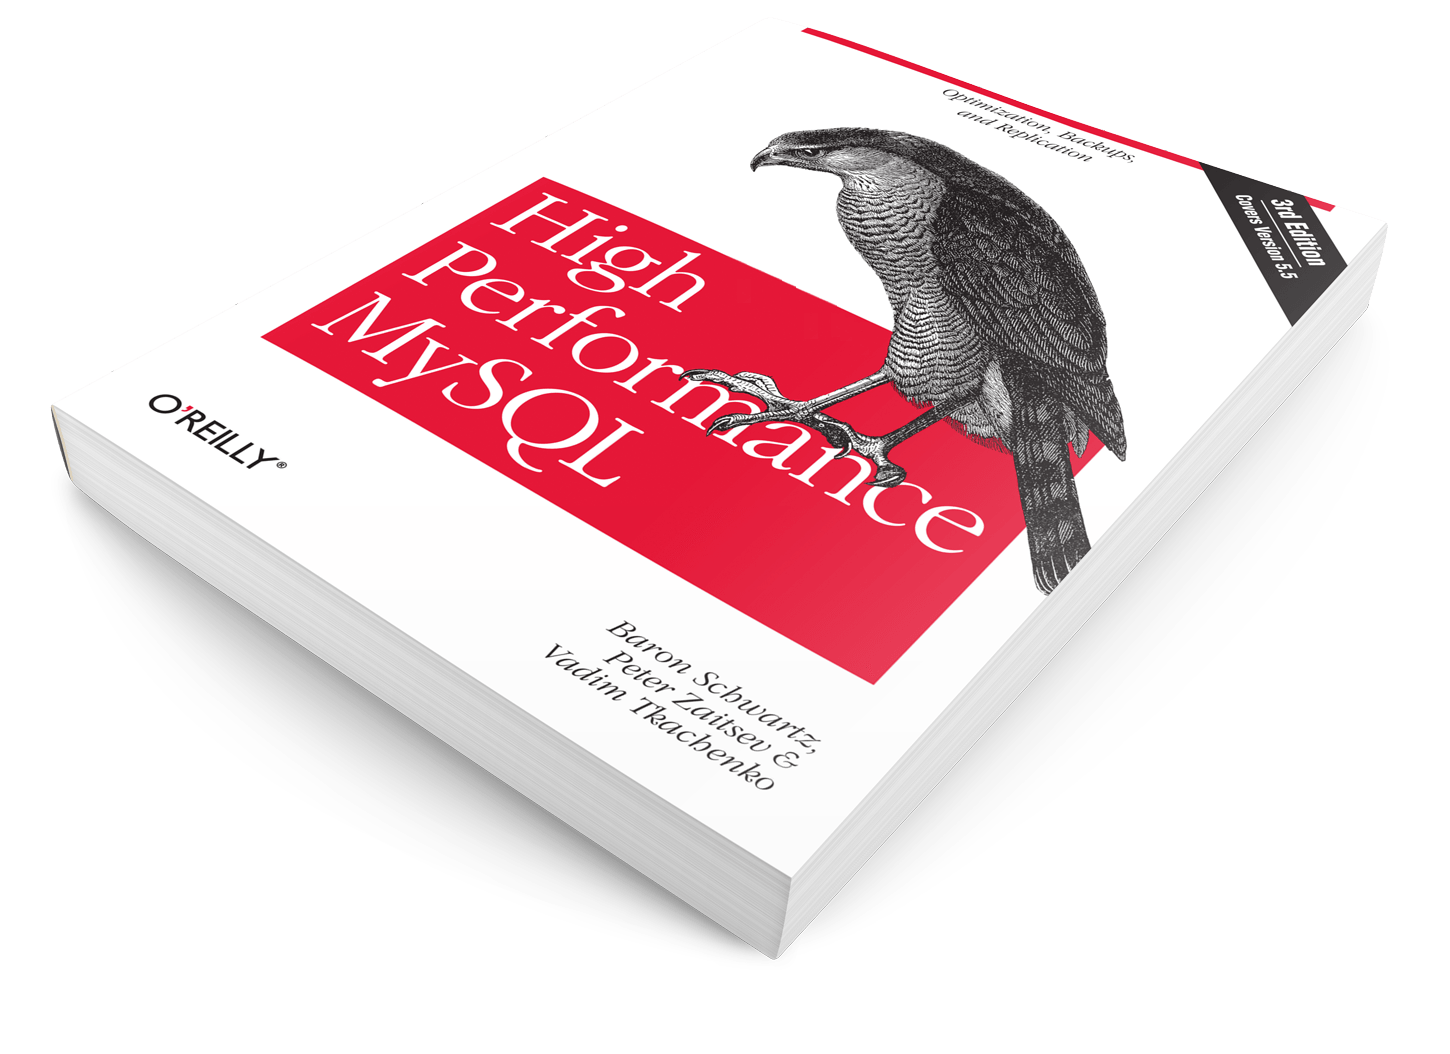
\includegraphics[width=9cm]{hpm-cover-perspective}
    \end{center}
}

\frame{
    \frametitle{Introduction}
    \framesubtitle{This Talk}

    \begin{enumerate}
        \item The Paper
        \item Computer Systems
        \item Nuclear Weapons
    \end{enumerate}
}

\frame{
    \frametitle{Introduction}
    \framesubtitle{Command and Control}

    \begin{center}
        
\includegraphics[height=7cm]{command-and-control}
    \end{center}
}

\frame{
    \frametitle{Introduction}
    \framesubtitle{Launch Complex 374-7, Little Rock Air Base, Arkansas}

    \begin{center}
        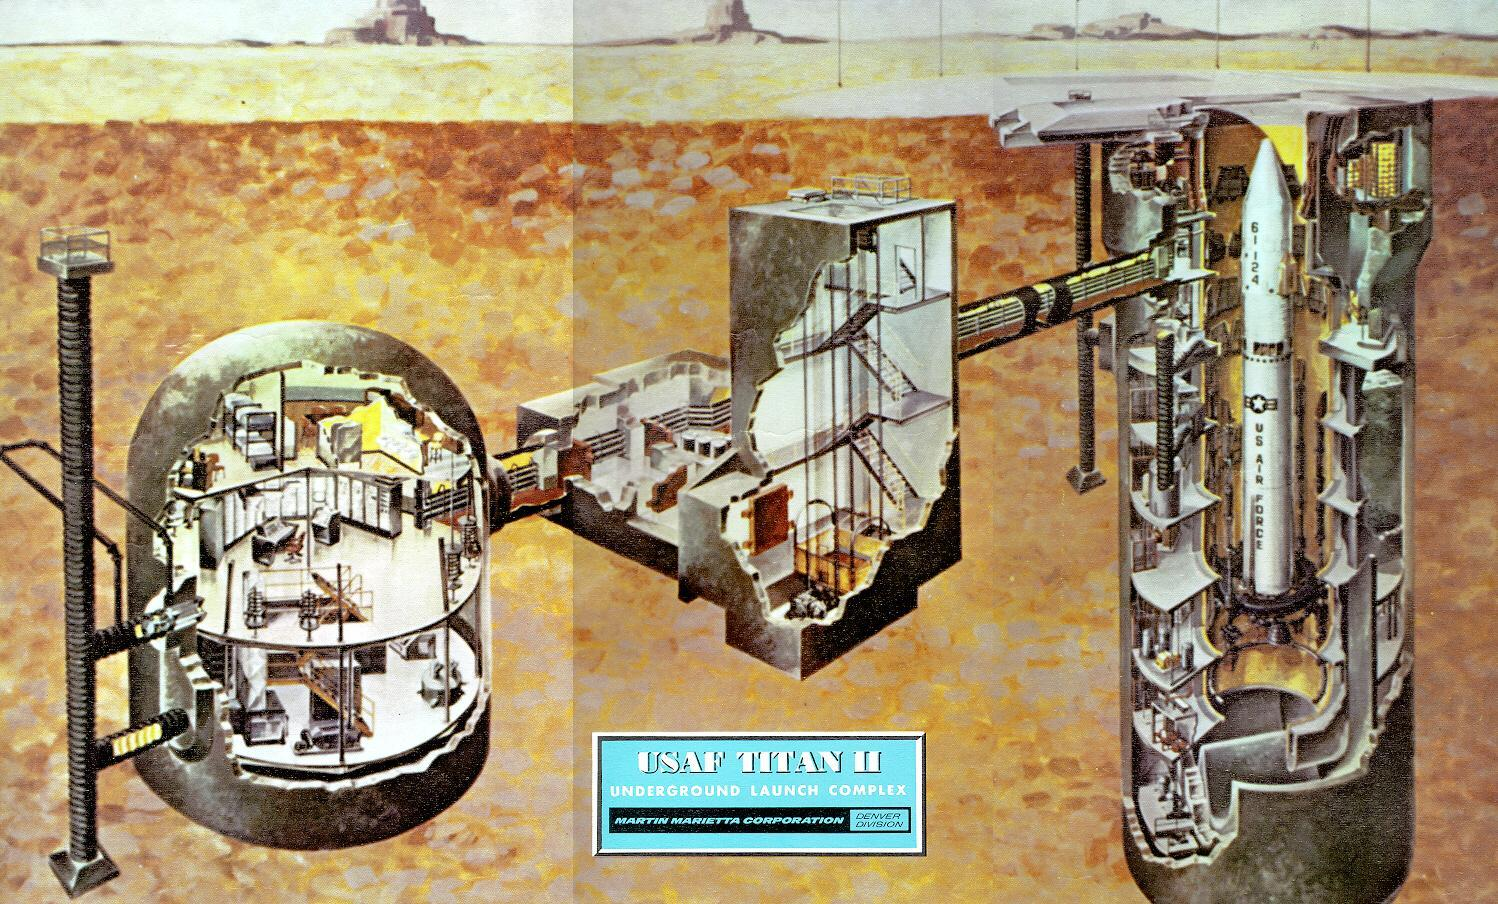
\includegraphics[width=10cm]{titan2bunker}
    \end{center}
}

\frame{
    \frametitle{Introduction}
    \framesubtitle{Launch Complex 374-7, Little Rock Air Base, Arkansas}

    \begin{center}
        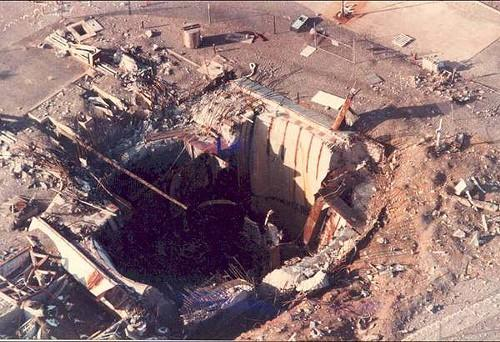
\includegraphics[width=10cm]{kaboom}
    \end{center}
}


% 1

\frame{
    \frametitle{1. Complex Systems are Intrinsically Hazardous Systems}

    \begin{itemize}
        \item Part of the definition
    \end{itemize}
}

\frame{
    \frametitle{1. Complex Systems are Intrinsically Hazardous Systems}
    \framesubtitle{Complex vs. Complicated}

    The Zen of Python states:

    \begin{itemize}
        \item Simple is better than complex.
        \item Complex is better than complicated.
    \end{itemize}
}

\frame{
    \frametitle{1. Complex systems are intrinsically hazardous systems.}
    \framesubtitle{Complex vs. Complicated}

    \begin{itemize}
        \item Complexity is intrinsic.
        \item Complication is extrinsic.
    \end{itemize}
}


% 2

\frame{
    \frametitle{2. Complex systems are heavily and successfully defended against failure.}

    \begin{itemize}
        \item Multiple layers
        \item \emph{Successful} = survivorship bias?
    \end{itemize}
}

% 4/5/6

\frame{
    \frametitle{4/5/6. Complex systems run on the edge of failure}

    ``Catastrophe is always just around the corner''

    \begin{itemize}
        \item There are always latent failures
    \end{itemize}
}


% 3/7/8

\frame{
    \frametitle{3/7/8. The Root Cause Fallacy}

    \textbf{Post-accident attribution to a `root cause' is fundamentally wrong.}

    \begin{itemize}
        \item Turtles all the way down to the CEO
        \item Hindsight bias
    \end{itemize}
}


\frame{
    \frametitle{3/7/8. The Root Cause Fallacy}

    \emph{``Hindsight bias remains the primary obstacle to accident investigation, especially when expert human performance is involved.''}

}

% 9/10

\frame{
    \frametitle{9/10. Human operators are producers of and defenders against failure who gamble}

    \begin{itemize}
        \item Unexpected Repercussions
        \item ``Try It''
    \end{itemize}
}


% 11

% 12/13/17

\frame{
    \frametitle{12/13/17. Human operators are the adaptable, but constantly changing, element}

    \begin{itemize}
        \item Celebrate the humanity
    \end{itemize}
}


% 14

\frame{
    \frametitle{14. Change introduces new forms of failure.}

    \begin{itemize}
        \item Reducing variability leads to ``black swans''
    \end{itemize}

    \begin{center}
        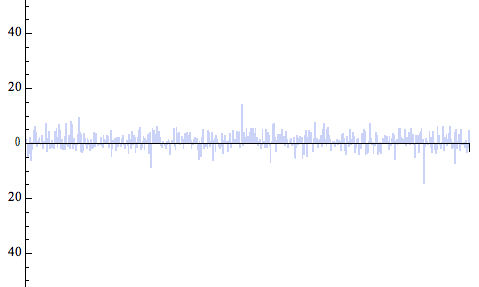
\includegraphics[width=5cm]{change-1}
        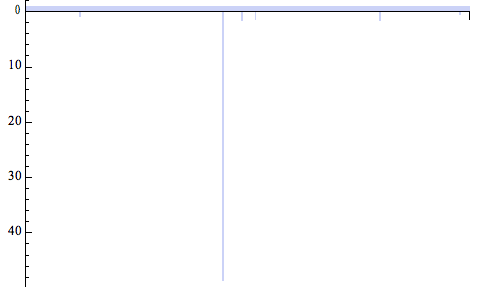
\includegraphics[width=5cm]{change-2}
    \end{center}
}

\frame{
    \frametitle{14. Change introduces new forms of failure.}

    \begin{description}
        \item[Iatrogenics] Harm caused by the healer
    \end{description}
}


% 16

\frame{
    \frametitle{16. Safety is a characteristic of systems and not of their components.}

    \begin{itemize}
        \item Take the holistic view
    \end{itemize}
}

\frame{
    \frametitle{16. Safety is a characteristic of systems and not of their components.}

    The Root Cause Fallacy again.
}


% Conclusion

\frame{
    \frametitle{Conclusion}

    \begin{itemize}
        \item Complex systems are hazardous, and run on the edge of failure
        \item Beware the root cause fallacy
        \item Value the human element
        \item Try really hard to not do iatrogenic harm
    \end{itemize}
}

\frame{
    \frametitle{Thank you}

    \begin{itemize}
        \item \url{me@adamj.eu}
    \end{itemize}
}


\end{document}
